The gain achieved using the Oracular Patent Query method motivated us to explore various methods to approximate the terms
selected by this query without ``peeking at the answers'' provided by
the actual relevance judgements.  We first attempt this via fully
automated methods and then proceed to evaluate semi-automated methods
based on interactive relevance feedback methods.

\subsection{Automated Reduction}
\label{sec:AutomatedReduction}
%\vspace*{-2ex}
%We noticed that most of the useful feedback terms exist in the original query and hypothesized that the baseline system could be substantially improved by removing negative query terms. 
%
% Why these approaches? provide citations for who has suggested them or otherwise
% provide a justification as to why each approach would be a good idea.  Do this
% in the bullet points where the actual method is discussed... not after the bullet
% points!  Don't dissociate content and discuss it multiple times in different
% places!  -Scott
We use the following four naive techniques to reduce the initial patent queries: 
%(i) removing Document Frequent terms (IDF(t)>$\tau$), (ii) keeping Frequent Terms in Query (QTF(t)>$\tau$); (iii) using Pseudo Relevance Feedback set (constructed after an initial run of the query) to select query terms (PRF(t)>$\tau$); and (iv) removing general terms in IPC title. 

\noindent \textbf{(1)-} In standard IR approaches, removing terms, appearing a lot in the collection, helps the retrieval effectiveness. Inspired by this fact, after an initial run of the query, we removed terms  with a Document Frequency (DF) in top-100 documents, higher than the threshold $\tau$. However, as illustrated in Figure \ref{fig:queryreduc}, it's clear that this technique significantly hurts the performance ($DF(t)>\tau$).  

\noindent \textbf{(2)-} Intuitivelly, frequent terms inside long and verbose queries are  important~\cite{maxwell2013compact}. Hence, we have  choosen to reduce queries by selecting terms with a frequency higher than a certain threshold $\tau$. The results in Figure \ref{fig:queryreduc} indicate clearly that this simple and naive technique is not adequate ($QTF(t)>\tau$). 

\noindent \textbf{(3)-} The third approach we experiment to reduce the query is based on Pseudo Relevance Feedback ($\mathit{PRF}$)~\cite{Baeza-Yates2011}. $\mathit{PRF}$ is an automated process without user interaction, which assumes the top k ranked documents are relevant. Again, it can be seen in Figure \ref{fig:queryreduc} that the results for query reduction using $\mathit{PRF}$ does not notably outperform the baseline. In fact, we could not find any heuristic correlates between  $ PRF(t)$ and $ RF(t)$. 
%Reda: Need clearly to be explained!}

\noindent \textbf{(4)-} Finally, we used words in IPC code title of each patent query to reduce the query, based on the assumption that they are common to all patents, which belong to the same category and may be considered as stop-words. However it did not help.
%we hurt the effectiveness by filtering them out.

% The anecdotal results and their implications have to be explained
% much more clearly... what is surprising about them (be specific:
% point out actual terms) and what can you take away from this
% investigation.  -Scott
Figure \ref{fig:anecdotal} shows an anecdotal example for a sample query about an invention related to ``emulsifier'', to explain why these four approaches fail. It shows the raw abstract, and a pair of terms and the associated $\mathit{RF}$ scores, where $t \in \{t| DF(t)/QTF(t)/PRF(t)>10\} $. It can be seen that the four methods fail clearly to discriminate between useful and noisy terms. As an example, terms like ``emulsifier'', ``maiz'' and ``amylas'' have been removed by the first method, which has probably led to decrease the quality of the query. As for the last method, it contains more noisy terms than useful terms (19 out of 32, and few of them with high negative score like ``saccharid'' or ``amylos''), but there are still some positive terms which we remove from the reference query that can prevent the system from a notable improvement.
%which resulted in bad retrieval performance. 
Therefore, this may suggest more sophisticated query reduction methods, as the one discussed in the next section.
 

%high scored terms are polluted with the sufficient amount of noise to hurt the retrieval effectiveness. Unfortunately, none of the proposed query reduction approaches for query reduction worked better than the baseline, which leads us to investigate interactive methods for reduction in the next section.

\subsection{Semi-automated Interactive Reduction}

\label{sec:SemiAutomatedInteractiveReduction}

%%%%%%%%%%%%%%%%%%%%%%%%%%%%%%%%%%%%%%%%%%%%%%%%%%%%%%%%%%%%
\begin{figure}[t!]
\begin{centering}
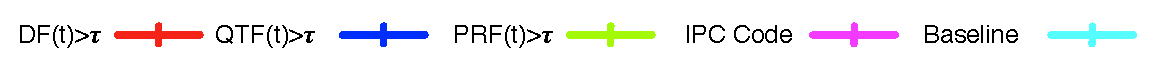
\includegraphics[width=9cm]{imgs/legend2}
\par\end{centering}

\begin{centering}
\subfigure[{Mean Average Precision.}]{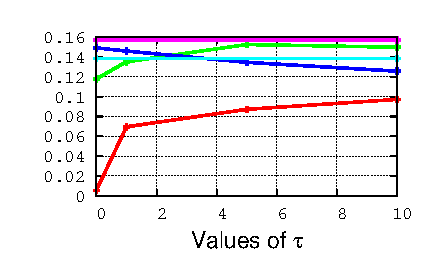
\includegraphics[width=4.5cm]{imgs/figure2-MAP}}\subfigure[Recall.]{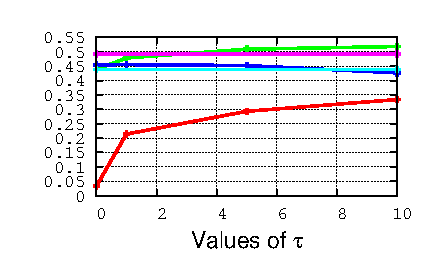
\includegraphics[width=4.5cm]{imgs/figure2-Recall}}
\par\end{centering}

\protect\caption{System performance vs. the threshold $\tau$ for four query reduction approaches.}
\label{fig:queryreduc}
\end{figure}
%%%%%%%%%%%%%%%%%%%%%%%%%%%%%%%%%%%%%%%%%%%%%%%%%%%%%%%%%%%%

%%%%%%%%%%%%%%%%%%%%%%%%%%%%%%%%%%%%%%%%%%%%%%%%%%%%%%%%%%%%
\begin{figure}[t!]
\begin{framed}
\vspace*{-2ex}
  \centering
    %\lstinputlisting[frame=single, basicstyle=\scriptsize\ttfamily , linewidth=\columnwidth,breaklines=true]{code/anecdotale.tex}\vspace*{-2ex}
 \begin{lstlisting}[basicstyle=\tiny\ttfamily , linewidth=\columnwidth,breaklines=true] 
PAC-1293
Abstract: The invention relates to an emulsifier, a method for
preparing said emulsifier, and to its use in various applications,
primarily food and cosmetic applications. The invention also relates 
to the use of said emulsifier for the creation of an elastic, gelled
foam. An emulsifier according to the invention is based on a starch
which is enzymatically converted, using a specific type of enzyme,
and modified in a specific esterification reaction.

DF Terms: <@\textcolor{blue}{starch:14.64}@>, <@\textcolor{blue}{enzym:29.49}@>, <@\textcolor{red}{amylos:-20.15}@>, <@\textcolor{blue}{oil:8.63}@>, <@\textcolor{red}{dispers:-8.66}@>,
<@\textcolor{red}{ph:-4.55}@>, <@\textcolor{red}{dry:-6.21}@>, <@\textcolor{red}{heat:-2.26}@>, <@\textcolor{red}{product:-5.48}@>, <@\textcolor{red}{slurri:-11.48}@>, <@\textcolor{blue}{viscos:7.77}@>,
<@\textcolor{red}{composit:-4.49}@>, <@\textcolor{red}{reaction:-1.97}@>, <@\textcolor{red}{food:-11.94}@>, <@\textcolor{blue}{agent:5.19}@>, <@\textcolor{red}{debranch:-10.58}@>, 
<@\textcolor{red}{reduc:-6.37}@>, <@\textcolor{red}{fat:-12.83}@>, <@\textcolor{red}{prepar:-0.82}@>, <@\textcolor{red}{hour:-5.42}@>, <@\textcolor{blue}{waxi:19.41}@>, <@\textcolor{blue}{deriv:11.97}@>, 
<@\textcolor{red}{content:-3.38}@>, <@\textcolor{blue}{aqueou:0.38}@>, <@\textcolor{red}{saccharid:-11.95}@>, <@\textcolor{red}{ml:-0.79}@>, <@\textcolor{red}{cook:-10.04}@>, <@\textcolor{blue}{modifi:5.65}@>, 
<@\textcolor{blue}{solid:5.50}@>, <@\textcolor{blue}{sampl:6.27}@>, <@\textcolor{blue}{mix:2.48}@>, <@\textcolor{red}{minut:-1.68}@>, <@\textcolor{red}{dri:-0.91}@>, <@\textcolor{red}{gel:-9.85}@>, 
<@\textcolor{blue}{activ:5.98}@>, <@\textcolor{red}{corn:-5.27}@>, <@\textcolor{blue}{alpha:12}@>, <@\textcolor{red}{sprai:-2.74}@> 

QTF Terms: <@\textcolor{blue}{starch:14.64}@>, <@\textcolor{blue}{emulsifi:6.72}@>, <@\textcolor{red}{succin:-3.46}@>, <@\textcolor{blue}{enzym:29.49}@>, <@\textcolor{blue}{emuls:12.66}@>, 
<@\textcolor{blue}{hydrophob:5.45}@>, <@\textcolor{red}{anhydrid:-5.47}@>, <@\textcolor{red}{reaction:-1.97}@>, <@\textcolor{red}{octenyl:-0.66}@>, <@\textcolor{blue}{stabil:3.64}@>, 
<@\textcolor{blue}{alkenyl:0.06}@>, <@\textcolor{blue}{reagent:1.17}@>, <@\textcolor{blue}{carbon:0.12}@>, <@\textcolor{blue}{potato:3.74}@>, <@\textcolor{red}{alkyl:-0.33}@>, <@\textcolor{red}{wt:-4.57}@>, 
<@\textcolor{blue}{ether:1.96}@>, <@\textcolor{red}{enzymat:-3.45}@>, <@\textcolor{blue}{convers:10.44}@>, <@\textcolor{red}{chain:-5.53}@>, <@\textcolor{blue}{atom:0.03}@>, <@\textcolor{red}{ph:-4.55}@>, 
<@\textcolor{red}{treat:-0.89}@>, <@\textcolor{red}{ammonium:-1.96}@>, <@\textcolor{red}{food:-11.94}@>, <@\textcolor{red}{amylos:-20.15}@>, <@\textcolor{red}{glucanotransferas:-0.86}@>, 
<@\textcolor{red}{glycidyl:-0.40}@>, <@\textcolor{red}{glycosyl:-0.02}@>, <@\textcolor{red}{dry:-6.21}@>, <@\textcolor{blue}{deriv:11.97}@>, <@\textcolor{blue}{transferas:0.89}@>, 
<@\textcolor{red}{foam:-0.49}@> 

PRF Terms: <@\textcolor{blue}{starch:14.64}@>, <@\textcolor{blue}{encapsul:17.50}@>, <@\textcolor{red}{chees:-4.22}@>, <@\textcolor{blue}{oil:8.63}@>, <@\textcolor{blue}{hydrophob:5.45}@>,
<@\textcolor{blue}{agent:5.19}@>, <@\textcolor{red}{casein:-2.19}@>, <@\textcolor{blue}{degrad:17.13}@>, <@\textcolor{blue}{deriv:11.97}@>, <@\textcolor{blue}{tablet:5.30}@>,
<@\textcolor{red}{debranch:-10.58}@>, <@\textcolor{red}{imit:-1.13}@>, <@\textcolor{blue}{viscos:7.77}@>, <@\textcolor{blue}{oxid:5.97}@>, <@\textcolor{blue}{activ:5.98}@>, <@\textcolor{blue}{osa:9.32}@>,
<@\textcolor{blue}{funnel:2.68}@>, <@\textcolor{blue}{amylas:26.06}@>, <@\textcolor{red}{amylopectin:-7.14}@>, <@\textcolor{blue}{maiz:20.61}@>, <@\textcolor{red}{blend:-3.17}@>, 
<@\textcolor{blue}{waxi:19.41}@>,   <@\textcolor{blue}{convert:31.81}@>

IPC def Terms: <@\textcolor{blue}{cosmet:3.77}@>, <@\textcolor{blue}{toilet:0.18}@>, <@\textcolor{red}{prepar:-0.82}@>, <@\textcolor{blue}{case:0.47}@>, 
<@\textcolor{red}{accessori:-0.01}@>, <@\textcolor{red}{store:-0.37}@>, <@\textcolor{blue}{handl:0.07}@>, <@\textcolor{red}{pasti:-0.17}@>, <@\textcolor{red}{substanc:-1.21}@>, 
<@\textcolor{red}{fibrou:-0.01}@>, <@\textcolor{red}{pulp:-1.28}@>, <@\textcolor{red}{constitut:-0.06}@>, <@\textcolor{blue}{paper:1.26}@>, <@\textcolor{red}{impregn:-0.11}@>, 
<@\textcolor{blue}{emulsifi:6.72}@>, <@\textcolor{red}{wet:-0.28}@>, <@\textcolor{red}{dispers:-8.66}@>, <@\textcolor{red}{foam:-0.49}@>, <@\textcolor{red}{produc:-0.57}@>, <@\textcolor{blue}{agent:5.19}@>, 
<@\textcolor{blue}{relev:0.18}@>, <@\textcolor{blue}{class:0.053}@>, <@\textcolor{red}{lubric:-0.38}@>, <@\textcolor{blue}{emuls:12.66}@>, <@\textcolor{red}{fuel:-0.011}@>, <@\textcolor{blue}{deriv:11.97}@>, 
<@\textcolor{blue}{starch:14.64}@>, <@\textcolor{red}{amylos:-20.15}@>, <@\textcolor{red}{compound:-0.63}@>, <@\textcolor{red}{saccharid:-11.95}@>, <@\textcolor{blue}{radic:1.03}@>, 
<@\textcolor{red}{acid:-3.19}@> 
 \end{lstlisting} 
 \vspace*{-2ex}
\end{framed}
 \vspace*{-2ex}
  \caption{Anecdotal example. Useful terms are highlighted in blue and the noisy ones in red.}
  \label{fig:anecdotal}  
\end{figure}
%%%%%%%%%%%%%%%%%%%%%%%%%%%%%%%%%%%%%%%%%%%%%%%%%%%%%%%%%%%%

Our anecdotal analysis of specific queries and terms selected via our oracular
approach suggests that automated methods fall far short of optimal term selection.
This leads us to explore another approach of approximating the oracular query
derived from relevance judgements by using a subset of relevance judgements
through interactive methods.  Specifically, to minimize the need for user interaction,
in this section we analyse the performance of an oracular query derived from
only the first relevant document identified in the search results.
\begin{comment}
All our attempts to improve the system effectiveness without accessing the relevance feedback were quite in vein because the features we recognized were tightly the combination of the useful words and noisy words and the system performance is too sensitive to the existence of a noisy word or the absence of the useful terms. So, we decided to apply much more realistic approach in which feedback terms are extracted only from the first ranked relevant document retrieved. 
\end{comment}
Using this approach, Table \ref{tab:firstrel} shows that we can double the MAP in comparison to our baseline and also outperform the PATATRAS system.

%%%%%%%%%%%%%%%%%%%%%%%%%%%%%%%%%%%%%%%%%%%%%%%%%%%%%%%%%%%%%%%%
\begin{table}[t!]
  \begin{center}
   \caption{System performance using minimal relevance feedback. $\tau$ is RF score threshold, and $k$ indicates the number of first relevant retrieved patents.}\vspace{3mm}
  \input table/partialRFtermselect.tex   
  \label{tab:firstrel}
  \end{center}  
\end{table}
%%%%%%%%%%%%%%%%%%%%%%%%%%%%%%%%%%%%%%%%%%%%%%%%%%%%%%%%%%%%%%%%

Furthermore, to establish the minimal interaction required by this
approach, Figure \ref{fig:FirstTPRankHisto} indicates that the
baseline methods return a relevant patent approximately 80\% of the
time in the first 10 results and 90\% of the time in the first 20
results.  Hence, such an interactive approach requires relatively low
user effort while achieving state-of-the-art performance.


\begin{figure}
\begin{centering}
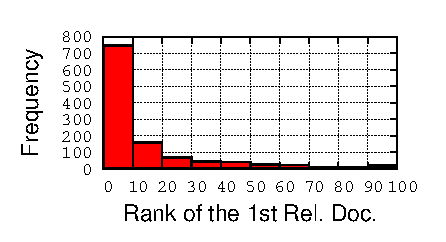
\includegraphics[width=5.5cm]{imgs/1stRank}
\par\end{centering}

\protect\caption{The distribution of the first relevant document rank over test queries.}
\label{fig:FirstTPRankHisto}
\end{figure}


